% WARIANCJA CUMSUM I ROZKLAD WYKLADNICZY, PODPISAC WYKRESY, 
% ??? sigma^0.5 symmetric? 
%  subplot dla sekwencji M i V

\documentclass[12pt, a4paper]{article}\usepackage[]{graphicx}\usepackage[]{color}
%% maxwidth is the original width if it is less than linewidth
%% otherwise use linewidth (to make sure the graphics do not exceed the margin)
\makeatletter
\def\maxwidth{ %
  \ifdim\Gin@nat@width>\linewidth
    \linewidth
  \else
    \Gin@nat@width
  \fi
}
\makeatother

\definecolor{fgcolor}{rgb}{0.345, 0.345, 0.345}
\newcommand{\hlnum}[1]{\textcolor[rgb]{0.686,0.059,0.569}{#1}}%
\newcommand{\hlstr}[1]{\textcolor[rgb]{0.192,0.494,0.8}{#1}}%
\newcommand{\hlcom}[1]{\textcolor[rgb]{0.678,0.584,0.686}{\textit{#1}}}%
\newcommand{\hlopt}[1]{\textcolor[rgb]{0,0,0}{#1}}%
\newcommand{\hlstd}[1]{\textcolor[rgb]{0.345,0.345,0.345}{#1}}%
\newcommand{\hlkwa}[1]{\textcolor[rgb]{0.161,0.373,0.58}{\textbf{#1}}}%
\newcommand{\hlkwb}[1]{\textcolor[rgb]{0.69,0.353,0.396}{#1}}%
\newcommand{\hlkwc}[1]{\textcolor[rgb]{0.333,0.667,0.333}{#1}}%
\newcommand{\hlkwd}[1]{\textcolor[rgb]{0.737,0.353,0.396}{\textbf{#1}}}%
\let\hlipl\hlkwb

\usepackage{framed}
\makeatletter
\newenvironment{kframe}{%
 \def\at@end@of@kframe{}%
 \ifinner\ifhmode%
  \def\at@end@of@kframe{\end{minipage}}%
  \begin{minipage}{\columnwidth}%
 \fi\fi%
 \def\FrameCommand##1{\hskip\@totalleftmargin \hskip-\fboxsep
 \colorbox{shadecolor}{##1}\hskip-\fboxsep
     % There is no \\@totalrightmargin, so:
     \hskip-\linewidth \hskip-\@totalleftmargin \hskip\columnwidth}%
 \MakeFramed {\advance\hsize-\width
   \@totalleftmargin\z@ \linewidth\hsize
   \@setminipage}}%
 {\par\unskip\endMakeFramed%
 \at@end@of@kframe}
\makeatother

\definecolor{shadecolor}{rgb}{.97, .97, .97}
\definecolor{messagecolor}{rgb}{0, 0, 0}
\definecolor{warningcolor}{rgb}{1, 0, 1}
\definecolor{errorcolor}{rgb}{1, 0, 0}
\newenvironment{knitrout}{}{} % an empty environment to be redefined in TeX

\usepackage{alltt}

%%%%%%%%%%%%%%%%%%%%%%%%%%%%%%%%%%%%%%%%%%%%%%%%%%%%%%%%%%%%%%%%
% LaTeX packages
%\usepackage[OT4]{polski}
\usepackage[utf8]{inputenc}
\usepackage[top=2.5cm, bottom=2.5cm, left=2cm, right=2cm]{geometry}
\usepackage{graphicx}
\usepackage{amsmath}
\usepackage{float}
\usepackage[colorlinks=true, linkcolor=blue]{hyperref}


%%%%%%%%%%%%%%%%%%%%%%%%%%%%%%%%%%%%%%%%%%%%%%%%%%%%%%%%%%%%%%%%
% global settings


\IfFileExists{upquote.sty}{\usepackage{upquote}}{}
\begin{document}

%%%%%%%%%%%%%%%%%%%%%%%%%%%%%%%%%%%%%%%%%%%%%%%%%%%%%%%%%%%%%%%%
% title page
\title{Estimation theory -- Laboratory 1.}
\author{Agnieszka Szkutek, 208619 \\ Marta Frankowska, 208581}
\maketitle
\tableofcontents 


%%%%%%%%%%%%%%%%%%%%%%%%%%%%%%%%%%%%%%%%%%%%%%%%%%%%%%%%%%%%%%%%
\section{Exercise 1}

We generate a vector of $Y\sim N(\mu=2, \sigma^2=4)$ with length $N = 1000$:
\begin{knitrout}
\definecolor{shadecolor}{rgb}{0.969, 0.969, 0.969}\color{fgcolor}\begin{kframe}
\begin{alltt}
\hlstd{Y} \hlkwb{<-} \hlkwd{rnorm}\hlstd{(}\hlkwc{n} \hlstd{=} \hlnum{1000}\hlstd{,} \hlkwc{mean} \hlstd{=} \hlnum{2}\hlstd{,} \hlkwc{sd} \hlstd{=} \hlnum{2}\hlstd{)}
\hlcom{# transform Y to Y1}
\hlstd{Y1} \hlkwb{<-} \hlnum{3} \hlopt{*} \hlstd{(Y} \hlopt{-} \hlnum{1}\hlstd{)}
\end{alltt}
\end{kframe}
\end{knitrout}
$Y_1$ has normal distribution, because it is a linear combination of $Y$. We can calculate analytical mean $\mu_1$ and variance $\sigma^2_1$:
\[ \mu_1 = E(Y_1) = E(3 (Y-1)) = 3 E(Y - 1) = 3 E(Y) - 3 = 3 \cdot 2 - 3 = 3\]
\[ \sigma^2_1 = Var(Y_1) = Var(3 (Y-1)) = 9 Var(Y) = 9 \cdot 4 = 36 \]

We can compare numerical and analytical results:
\begin{knitrout}
\definecolor{shadecolor}{rgb}{0.969, 0.969, 0.969}\color{fgcolor}\begin{kframe}
\begin{alltt}
\hlstd{Y} \hlkwb{<-} \hlkwd{rnorm}\hlstd{(}\hlkwc{n} \hlstd{=} \hlnum{1000}\hlstd{,} \hlkwc{mean} \hlstd{=} \hlnum{2}\hlstd{,} \hlkwc{sd} \hlstd{=} \hlnum{2}\hlstd{)}
\hlstd{Y1} \hlkwb{<-} \hlnum{3} \hlopt{*} \hlstd{(Y} \hlopt{-} \hlnum{1}\hlstd{)}
\hlkwd{mean}\hlstd{(Y1)}
\end{alltt}
\begin{verbatim}
## [1] 3.047471
\end{verbatim}
\begin{alltt}
\hlkwd{var}\hlstd{(Y1)}
\end{alltt}
\begin{verbatim}
## [1] 34.70353
\end{verbatim}
\end{kframe}
\end{knitrout}

Now we can plot the frequency historam of $Y_1$ and analytical normal density with $\mu=3$ and $\sigma^2=36$.
\begin{knitrout}
\definecolor{shadecolor}{rgb}{0.969, 0.969, 0.969}\color{fgcolor}

{\centering 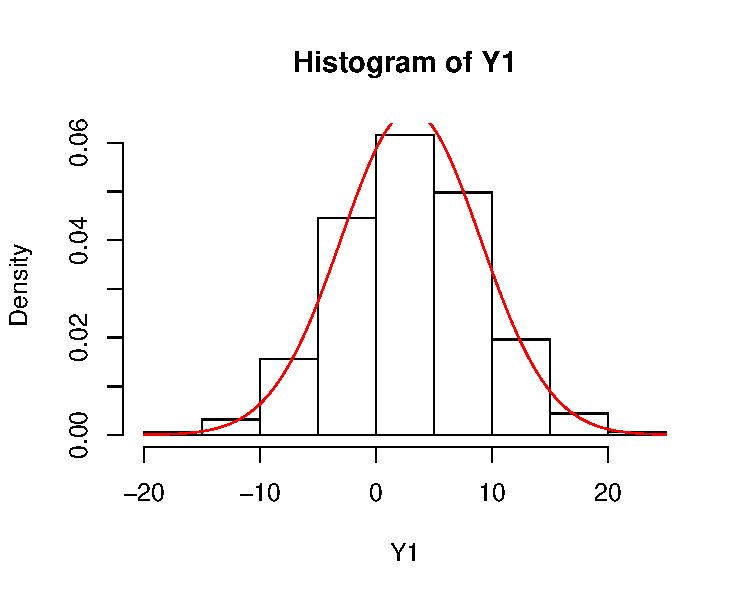
\includegraphics[width=\maxwidth]{figure/ex1_1hist-1} 

}



\end{knitrout}

Next, we create variable $Y_2$
\[ Y_2 = \left( \frac{Y_1-2}{2} \right)^2 \]
and plot its frequency historam.
\begin{knitrout}
\definecolor{shadecolor}{rgb}{0.969, 0.969, 0.969}\color{fgcolor}\begin{kframe}
\begin{alltt}
\hlstd{Y} \hlkwb{<-} \hlkwd{rnorm}\hlstd{(}\hlkwc{n} \hlstd{=} \hlnum{1000}\hlstd{,} \hlkwc{mean} \hlstd{=} \hlnum{2}\hlstd{,} \hlkwc{sd} \hlstd{=} \hlnum{2}\hlstd{)}
\hlstd{Y1} \hlkwb{<-} \hlnum{3} \hlopt{*} \hlstd{(Y} \hlopt{-} \hlnum{1}\hlstd{)}
\hlstd{Y2} \hlkwb{<-} \hlstd{((Y1} \hlopt{-} \hlnum{2}\hlstd{)} \hlopt{/} \hlnum{2}\hlstd{)} \hlopt{^} \hlnum{2}

\hlkwd{hist}\hlstd{(Y2,} \hlkwc{freq} \hlstd{=} \hlnum{FALSE}\hlstd{)}
\end{alltt}
\end{kframe}

{\centering 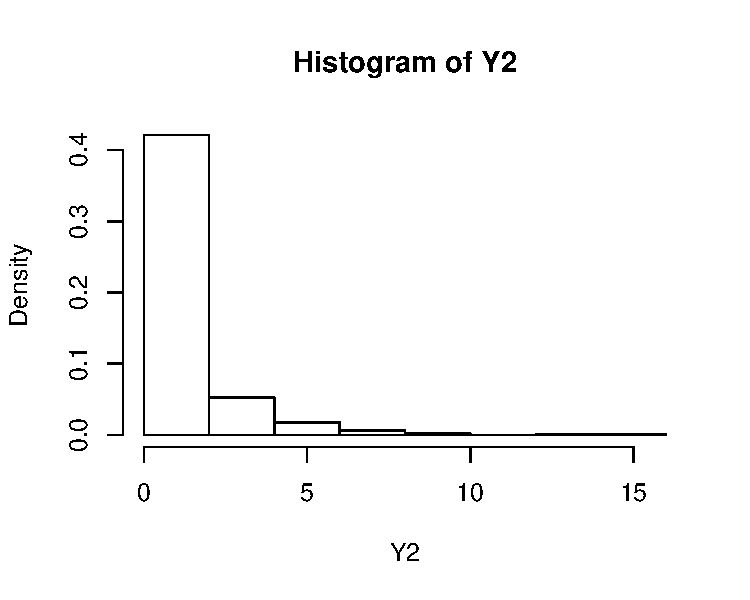
\includegraphics[width=\maxwidth]{figure/ex1_2-1} 

}



\end{knitrout}

$Y_2$ is a quadratic function of $Y_1$, so we know that distribution of $Y_2$ is not normal. From the shape histogram we can assume that $Y_2$ has exponential distribution with 
\[\lambda = \frac{1}{E(Y_2)}.\]

We can obtain the analytical value of $E(Y_2)$ in the following way
\begin{align*}
E(Y_2)=& E\left(\left( \frac{Y_1-2}{2} \right)^2\right) = \frac{1}{4} E(Y_1-2)^2 = \frac{1}{4} E(Y_1^2 - 2Y_1 +4) =  \\ 
=& \frac{1}{4} EY_1^2 - \frac{1}{2} E Y_1 + 1= \frac{1}{4}\left(Var Y_1 +(E Y_1)^2\right)-\frac{1}{2} E Y_1 + 1 = \\
=& \frac{1}{4} (36 + 9) - \frac{3}{2} + 1 = 10.75,
\end{align*}

so $\lambda = \frac{1}{10.75}\approx 0.093$.

\begin{knitrout}
\definecolor{shadecolor}{rgb}{0.969, 0.969, 0.969}\color{fgcolor}

{\centering 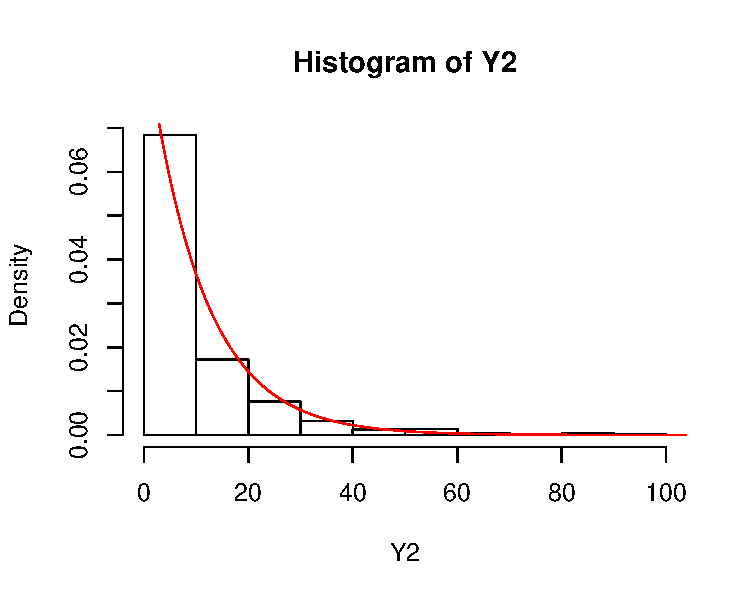
\includegraphics[width=\maxwidth]{figure/ex1_2hist-1} 

}



\end{knitrout}
Next we will compute a sequence of means $m_n$ and a sequence of variances $\sigma_n^2$ for the variable~$Y$, where
\[ m_n = \frac{1}{n} \sum_{i=1}^{n} Y_i \]
\[ \sigma_n = \frac{1}{n} \sum_{i=1}^{n} (Y_i - m_n)^2 \]
and plot the results.

\begin{knitrout}
\definecolor{shadecolor}{rgb}{0.969, 0.969, 0.969}\color{fgcolor}

{\centering 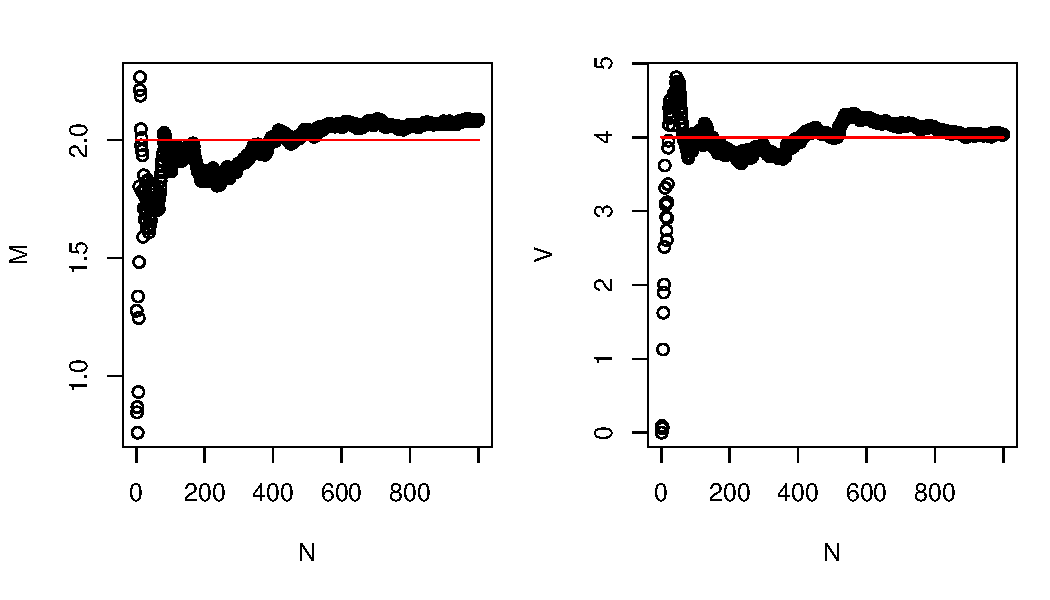
\includegraphics[width=\maxwidth]{figure/ex1_2seq-1} 

}



\end{knitrout}

The sequences $m_n$ and $\sigma_n^2$ converge to theoretical mean and variance, respectively. To examine the variability of the sequences we can calculate relative errors for both values.

\[ err_{M_n} = \left| \frac{M_n - \mu_n}{\mu_n}  \right| \]

\begin{knitrout}
\definecolor{shadecolor}{rgb}{0.969, 0.969, 0.969}\color{fgcolor}

{\centering 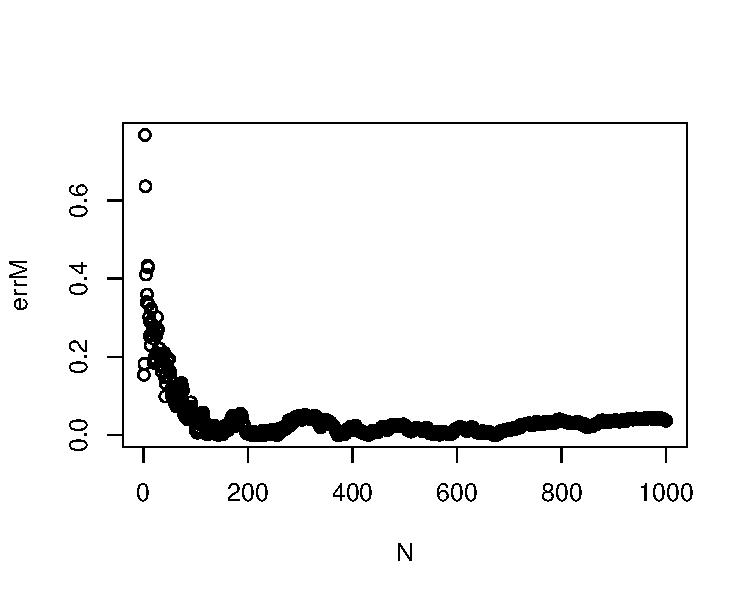
\includegraphics[width=\maxwidth]{figure/ex1_2err-1} 

}



\end{knitrout}

For $N>200$ value of the error is less than $10\%$ of theoretical mean.
















%%%%%%%%%%%%%%%%%%%%%%%%%%%%%%%%%%%%%%%%%%%%%%%%%%%%%%%%%%%%%%%%
\section{Exercise 2}

We simulate 10000 times and then plot 2-dimensional random variable $X\sim N(0,I_2)$.

\begin{knitrout}
\definecolor{shadecolor}{rgb}{0.969, 0.969, 0.969}\color{fgcolor}\begin{kframe}
\begin{alltt}
\hlstd{n} \hlkwb{<-} \hlnum{10000}
\hlstd{mu} \hlkwb{<-} \hlkwd{c}\hlstd{(}\hlnum{0}\hlstd{,} \hlnum{0}\hlstd{)}
\hlstd{Sigma} \hlkwb{<-} \hlkwd{diag}\hlstd{(}\hlnum{2}\hlstd{)}
\hlstd{X} \hlkwb{<-} \hlkwd{rmvnorm}\hlstd{(}\hlkwc{n} \hlstd{= n,} \hlkwc{mean} \hlstd{= mu,} \hlkwc{sigma} \hlstd{=  Sigma)}
\hlkwd{plot}\hlstd{(X)}
\end{alltt}
\end{kframe}

{\centering 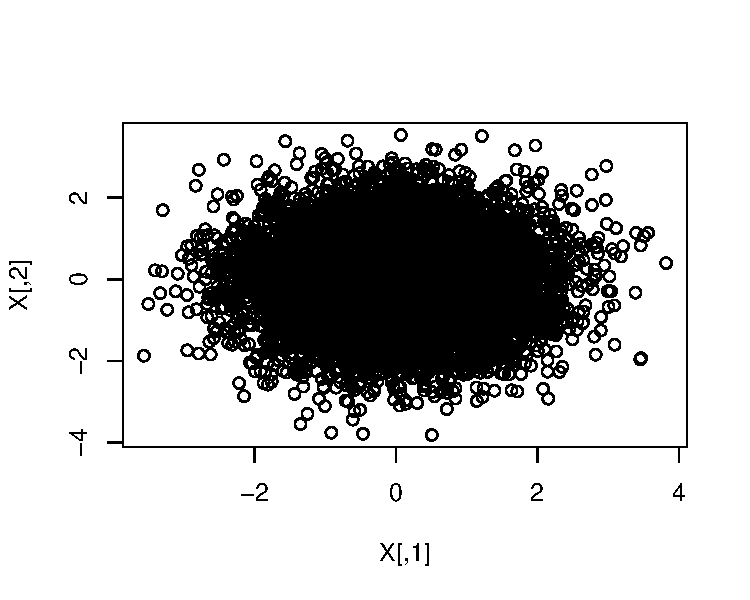
\includegraphics[width=\maxwidth]{figure/ex2X-1} 

}



\end{knitrout}

We have to transform variable $X$ into variable $Y \sim N(\mu, \Sigma)$, where 
\[\mu = \left[0,\ 1\right] \quad \text{and }\quad 
  \Sigma = \left[
    \begin{matrix}  
      2   & 0.5 \\
      0.5 & 2
    \end{matrix} 
    \right]
\]
It means that we should find vector $a$ and matrix $A$, such that $Y=A X + a$. 

% From the lecture we know that if 
% \[ X\sim N(0, I_2), \quad Y\sim N(\mu, \Sigma) \quad \text{and }\quad Y = AX + b,\] 
% then 
% \[Y = \Sigma^{0.5}X + \mu. \] 

Expected value of $Y$ is equal to
\[E(Y) = E(AX+a) = A E(X)+a = a, \]
and variance
\[Var(Y) = Var(AX+a) = Var(AX) = A Var(X) A' = A I A' = A A' = \Sigma = \Sigma^{0.5} \left(\Sigma^{0.5}\right)'. \]
From that we obtain $A = \Sigma^{0.5}$, so 
\[ Y = \Sigma^{0.5}X + \mu.  \]
% \[ A = \Sigma^{0.5}\] \quad \text{and }\quad a = \mu. \]

\begin{knitrout}
\definecolor{shadecolor}{rgb}{0.969, 0.969, 0.969}\color{fgcolor}\begin{figure}[H]

{\centering 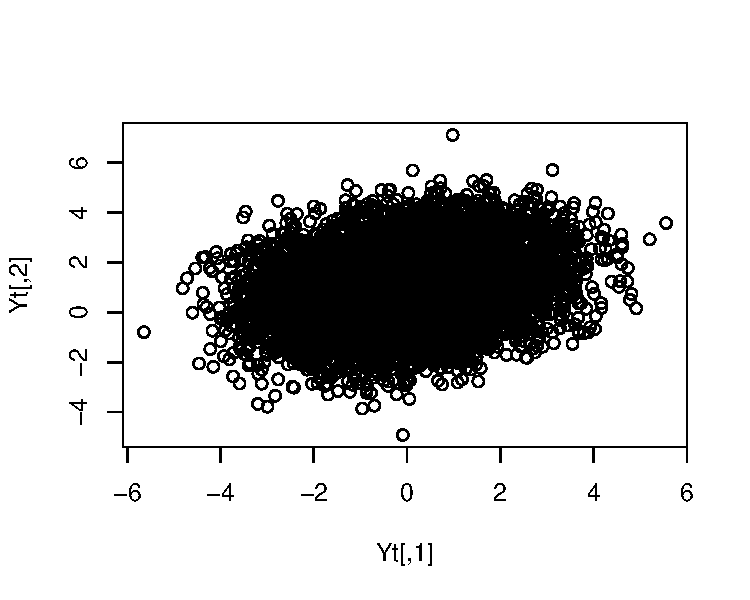
\includegraphics[width=\maxwidth]{figure/ex2Y-1} 

}

\caption[Random variable $Y$]{Random variable $Y$}\label{fig:ex2Y}
\end{figure}


\end{knitrout}

\begin{knitrout}
\definecolor{shadecolor}{rgb}{0.969, 0.969, 0.969}\color{fgcolor}\begin{kframe}


{\ttfamily\noindent\bfseries\color{errorcolor}{\#\# Error in eval(expr, envir, enclos): could not find function "{}hist3D"{}}}\end{kframe}
\end{knitrout}

\begin{knitrout}
\definecolor{shadecolor}{rgb}{0.969, 0.969, 0.969}\color{fgcolor}\begin{kframe}
\begin{alltt}
\hlstd{n} \hlkwb{<-} \hlnum{10000}
\hlstd{mu} \hlkwb{<-} \hlkwd{c}\hlstd{(}\hlnum{0}\hlstd{,} \hlnum{0}\hlstd{)}
\hlstd{Sigma} \hlkwb{<-} \hlkwd{diag}\hlstd{(}\hlnum{2}\hlstd{)}
\hlstd{X} \hlkwb{<-} \hlkwd{rmvnorm}\hlstd{(}\hlkwc{n} \hlstd{= n,} \hlkwc{mean} \hlstd{= mu,} \hlkwc{sigma} \hlstd{=  Sigma)}
\hlkwd{plot}\hlstd{(X)}
\end{alltt}
\end{kframe}

{\centering 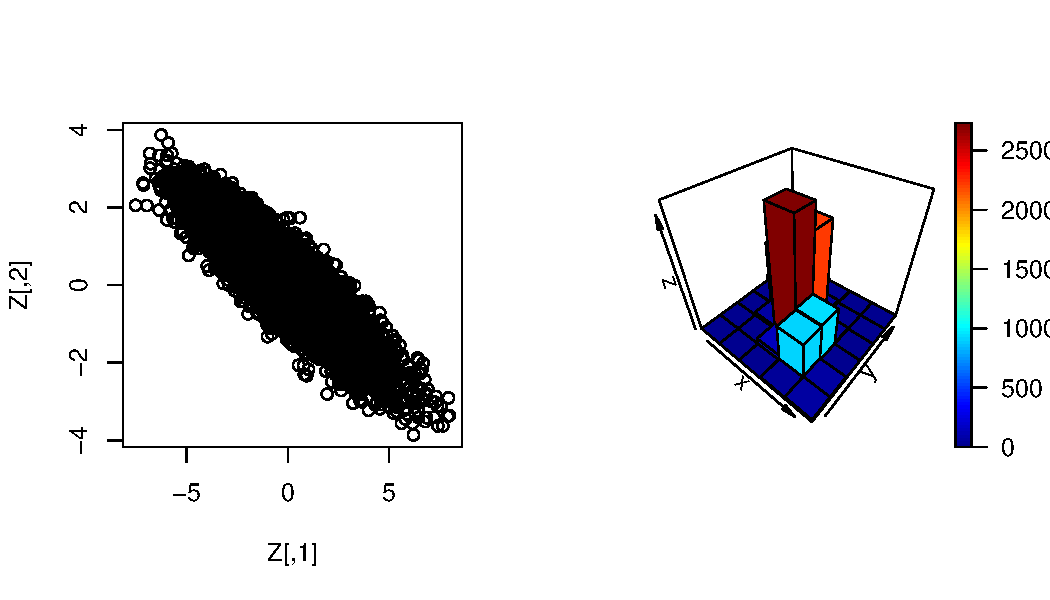
\includegraphics[width=\maxwidth]{figure/ex2histZ-1} 

}



\end{knitrout}












%%%%%%%%%%%%%%%%%%%%%%%%%%%%%%%%%%%%%%%%%%%%%%%%%%%%%%%%%%%%%%%%
\section{Exercise 3}













%%%%%%%%%%%%%%%%%%%%%%%%%%%%%%%%%%%%%%%%%%%%%%%%%%%%%%%%%%%%%%%%
When using additional source materials (books, links, etc.)
do not forget to include appropriate references.  For example, let us assume 
we want to cite Dalgard (2008). Then the bibliography section should contain:

\begin{thebibliography}{}
 
\bibitem{Dalgard2008}
  Peter Dalgaard, \emph{Introductory Statistics with R}, Springer-Verlag New York, 2008.

\end{thebibliography}

\end{document}
